\documentclass[notheorems,mathserif,table,compress]{beamer}  %dvipdfm选项是关键,否则编译统统通不过
%%------------------------常用宏包------------------------
%%注意, beamer 会默认使用下列宏包: amsthm, graphicx, hyperref, color, xcolor, 等等
\usepackage{fontspec,xunicode,xltxtra}  % for XeTeX
\usepackage{verbatim}
\usepackage{mathabx}
\usepackage{amsfonts,amssymb}
\usepackage{iplouclistings}
\usepackage{fancybox}
\usepackage{colortbl}
\usepackage{tcolorbox}
\usepackage[absolute,overlay]{textpos}
%%------------------------ThemeColorFont------------------------
%% Presentation Themes
% \usetheme[<options>]{<name list>}
\usetheme{Madrid}
%% Inner Themes双精度计算
% \useinnertheme[<options>]{<name>}
%% Outer Themes
% \useoutertheme[<options>]{<name>}
\useoutertheme{miniframes} 
%% Color Themes 
%\usecolortheme[<options>]{<name list>}
%% Font Themes
\usefonttheme{serif}
\setbeamertemplate{background canvas}[vertical shading][bottom=white,top=structure.fg!7] %%背景色, 上25%的蓝, 过渡到下白.
\setbeamertemplate{theorems}[numbered]
\setbeamertemplate{navigation symbols}{}   %% 去掉页面下方默认的导航条.
\usepackage{zhfontcfg}
%\setsansfont[Mapping=tex-text]{文泉驿正黑}  %% 需要fontspec宏包
     %如果装了Adobe Acrobat,可在font.conf中配置Adobe字体的路径以使用其中文字体
     %也可直接使用系统中的中文字体如SimSun,SimHei,微软雅黑 等
     %原来beamer用的字体是sans family;注意Mapping的大小写,不能写错
     %设置字体时也可以直接用字体名,以下三种方式等同:
     %\setromanfont[BoldFont={黑体}]{宋体}
     %\setromanfont[BoldFont={SimHei}]{SimSun}
     %\setromanfont[BoldFont={"[simhei.ttf]"}]{"[simsun.ttc]"}
%%------------------------MISC------------------------
\graphicspath{{figures/}}         %% 图片路径. 本文的图片都放在这个文件夹里了.
%%------------------------正文------------------------
\begin{document}
\XeTeXlinebreaklocale "zh"         % 表示用中文的断行
\XeTeXlinebreakskip = 0pt plus 1pt % 多一点调整的空间
%%----------------------------------------------------------
%% This is only inserted into the PDF information catalog. Can be left
%% out.
%%%
%% Delete this, if you do not want the table of contents to pop up at
%% the beginning of each subsection:
\AtBeginSection[]{                              % 在每个Section前都会加入的Frame
  \frame<handout:0>{
    \frametitle{Contents}\small
    \tableofcontents[current,currentsubsection]
  }
}

\AtBeginSubsection[]                            % 在每个子段落之前
{
  \frame<handout:0>                             % handout:0 表示只在手稿中出现
  {
    \frametitle{Contents}\small
    \tableofcontents[current,currentsubsection] % 显示在目录中加亮的当前章节
  }
}

%%----------------------------------------------------------
\title{Learning-Based PDE in Computer Vision}
%\subtitle{Total variation denoising-ROF model}
\author[Qiu]{主讲人~~~~~\textcolor{olive}{邱欣欣}\\
    \quad 幻灯片制作~~\textcolor{olive}{邱欣欣}}
\institute[中国海洋大学]{\small\textcolor{violet}{中国海洋大学~~信息科学与工程学院}}
\date{2014~年~10~月~31~日}
%\titlegraphic{\vspace{-6em}\includegraphics[height=7cm]{ouc}\vspace{-6em}}
\frame{ \titlepage }
%%----------------------------------------------------------
\section*{Contents}
\frame{\frametitle{Learning-Based PDE in Computer Vision}\tableofcontents}
%%----------------------------------------------------------
\section{Adaptive PDE Learning for Visual Saliency Detection}

%
\begin{frame}
\frametitle{Adaptive PDE Learning for Visual Saliency Detection}
主要内容:显著度检测的自适应PDE学习方法\\
背景:
\begin{itemize}
\item 传统的PDE方法:一般应用于处理低层的视觉问题,如图像去噪等;固定的形式与边界条件难以处理复杂的视觉任务。
\item PDE+Learning :扩散的观点来理解和模拟显著度检测的物理性质;结合自底向上,自顶向下的先验知识;提出LESD模型,并有效求解。
\end{itemize}
\end{frame}

%
\begin{frame}
\frametitle{显著度检测与扩散}
扩散:物理意义,扩散方程,图像去噪\\
显著度检测是一个从图像中检测出最能吸引人的视觉注意的物体区域的计算机视觉处理过程。\\
这个过程可以用扩散的观点来看:假设我们的注意首先被最典型的显著的图像元素(文章中为显著性种子)所吸引,然后视觉注意会扩散到整个显著区域。
\end{frame}

%\section{}

%
\begin{frame}
\frametitle{LESD(Linear Elliptic System with Dirichlet Boundary)}
定义扩散过程:
\begin{displaymath}
\frac{\partial f(\mathbf{p},t)}{\partial t}=F(f,\nabla f), \;f(g)=0,\;f(\mathbf{p})=s_\mathbf{p},\;\mathbf{p}\in S
\end{displaymath}

其中实值得分函数(real-value visual attention score function)$f(\mathbf{p})$衡量了$p$的显著度($p\in \nu$,$\nu$是图像域).\\
\emph{假设已知显著度种子的集合(S)和它相应的初始分数$f(\mathbf{p})=s_\mathbf{p},\mathbf{p}\in S$。}

\begin{displaymath}
F(f,\nabla f)=\mathrm{div}(\mathbf{K_p}\nabla f(p))+\lambda(f(\mathbf{p})-g(\mathbf{p}))
\end{displaymath}

引入正则化项$f(\mathbf{p})$与Guidance map $g(\mathbf{p})$的差。\\
\emph{对于扩散方程来说,当显著注意不再扩散,显著度过程达到稳定,此时$F(f,\nabla f)=0$。这时对方程进行离散化处理可以得到$f(p)$的表达式。}
\end{frame}

%
\begin{frame}
\frametitle{Learning LESD for Saliency Detection}
\begin{itemize}
\item<1-> 建立的LESD模型与Learning有什么关系?学习的是什么?
\item<2-> 学习的是Guidance map (g(p))与边界条件(saliency seeds 集S)
\item<3->学习是求解PDE的参数
\end{itemize}

\end{frame}

%
\begin{frame}
%\frametitle{}
\begin{figure}
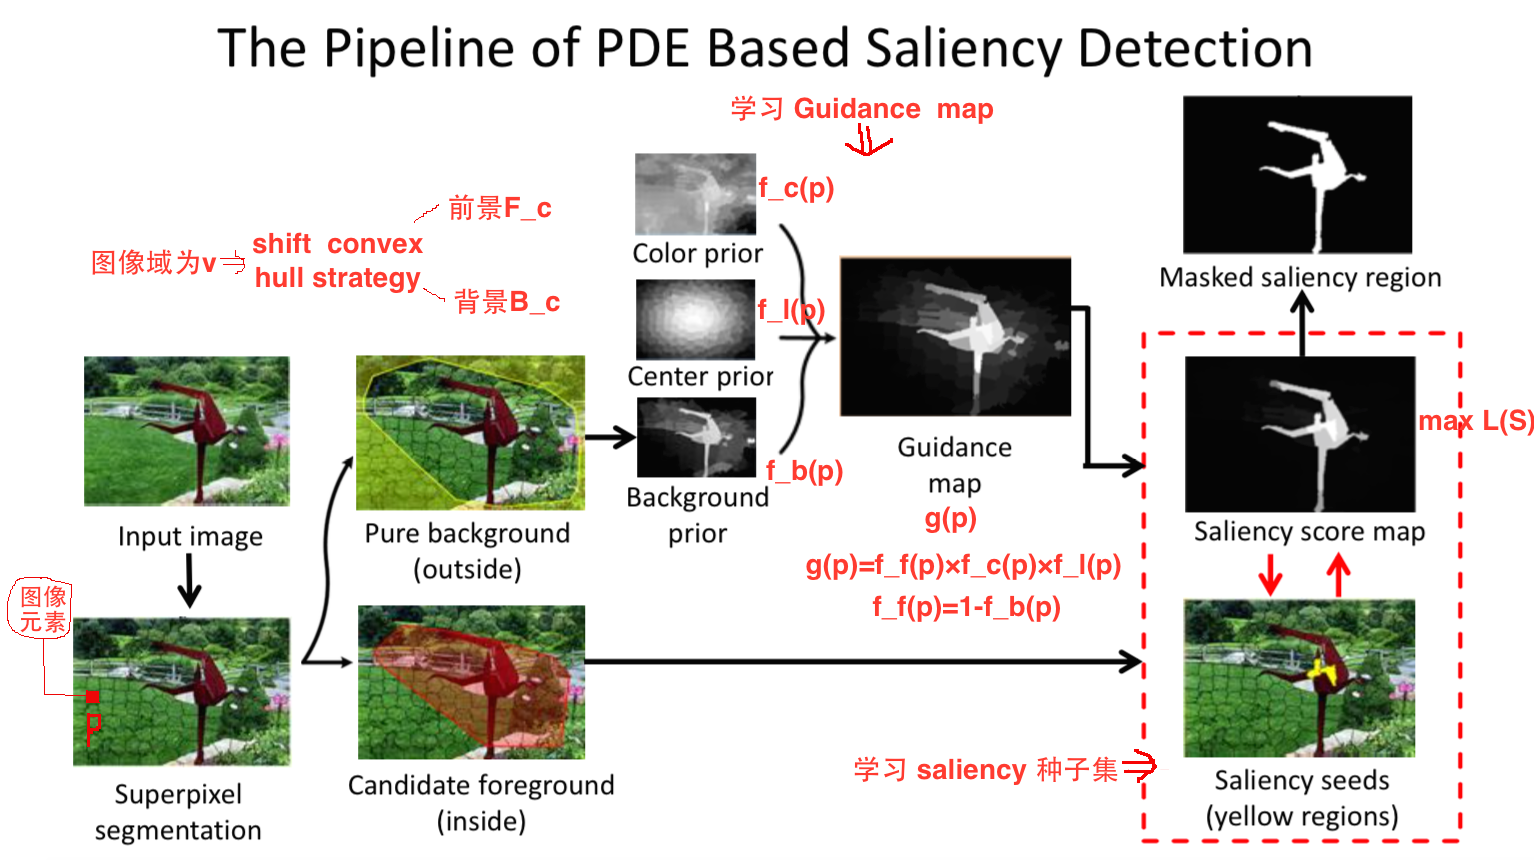
\includegraphics[width=12.5cm]{pipeline.png}
\end{figure}

\end{frame}

%
\begin{frame}
\frametitle{Learning boundary conditions(S)}
如何选择显著度扩散的种子点?\\
-不能选择前景中所有的点作为显著度扩散的种子。
\begin{itemize}
\item  前景中含有背景的点。
\item 可以观察到和领域有髙局部对比度的种子(邻近边界的点和亮、暗的点)可能会导致得到较差的显著图。
\end{itemize}

-目标是将种子的视觉注意得分扩散到整个图像域$\nu$。\\
因此可以通过求得$\nu$中全部图像元素得分的和的极大值来定义种子集$S$。

\end{frame}

%
\begin{frame}
\frametitle{Learning boundary conditions(S)}
以上问题简化为下列的离散最优化问题
\begin{equation*}
\begin{split}
&\max_{S\in \mathbb{M}^n}L(S)\\
&s.t.\bigg{\{}\begin{array}{ll}
f(\mathbf{p})=\frac{1}{d_p+\lambda}(\sum_{\mathbf{q}\in N(\mathbf{p})})\mathbf{K_p(q)}f(\mathbf{q})+\lambda g(\mathbf{p}))\\
f(g)=0,\;f(\mathbf{p})=s_\mathbf{p},\;\mathbf{p}\in S
\end{array} 
\end{split}
\end{equation*}

其中$L(S)=\sum_{\mathbf{p}\in \nu}f(\mathbf{p};S),\mathbb{M}^n=\{S|S\subset F_c,|S|\leq n\}$。\\
分数可以看做点与种子间的关系,因此前景内有髙局部对比度的点将会从$S$中移除;在前景内的背景点有相对较小的$L$值,因此也不在$S$里面。\\
但结果依赖于显著度种子集$S$的最大数量$n$,作者采用了一种自适应的选择方法来判断n并且进一步去除了$F_c$中的背景点。
\end{frame}

%
\begin{frame}
\frametitle{ 最终结果}
得到了Guidance map,种子集$S$,便可以求解$f(p)$了,由$f(p)$可以构造出最终的显著图。

\end{frame}

\section{Learning a general PDE system for computer vision}

%
\begin{frame}
\frametitle{general PDE system}
大多数对一幅图像$u$处理的PDE可以写作下列的形式:
\begin{displaymath}
\frac{\partial u}{\partial t}-F(u,\nabla u,\mathbf{H}_u)=0
\end{displaymath}

%如何与学习联系起来?

\end{frame}

%
\begin{frame}
\frametitle{general PDE system}
\begin{figure}
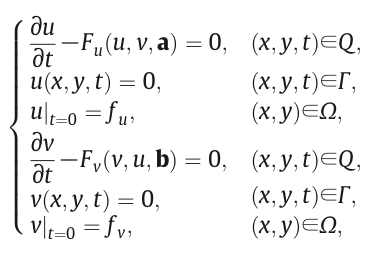
\includegraphics[width=6cm]{gong.png}
\end{figure}
\begin{figure}
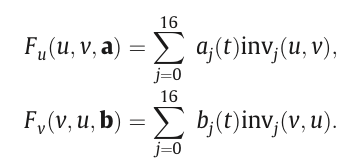
\includegraphics[width=6cm]{gong1.png}
\end{figure}

\end{frame}

%
\begin{frame}
\frametitle{general PDE system}
如何与学习联系起来?
\begin{itemize}
\item 表示平移旋转微分不变性质的“字典”。
\item 建立PDE方程学习系数函数a,b,这个模型的求解是一个训练过程
\end{itemize}

\end{frame}

%
\begin{frame}
\frametitle{general PDE system}
\begin{figure}
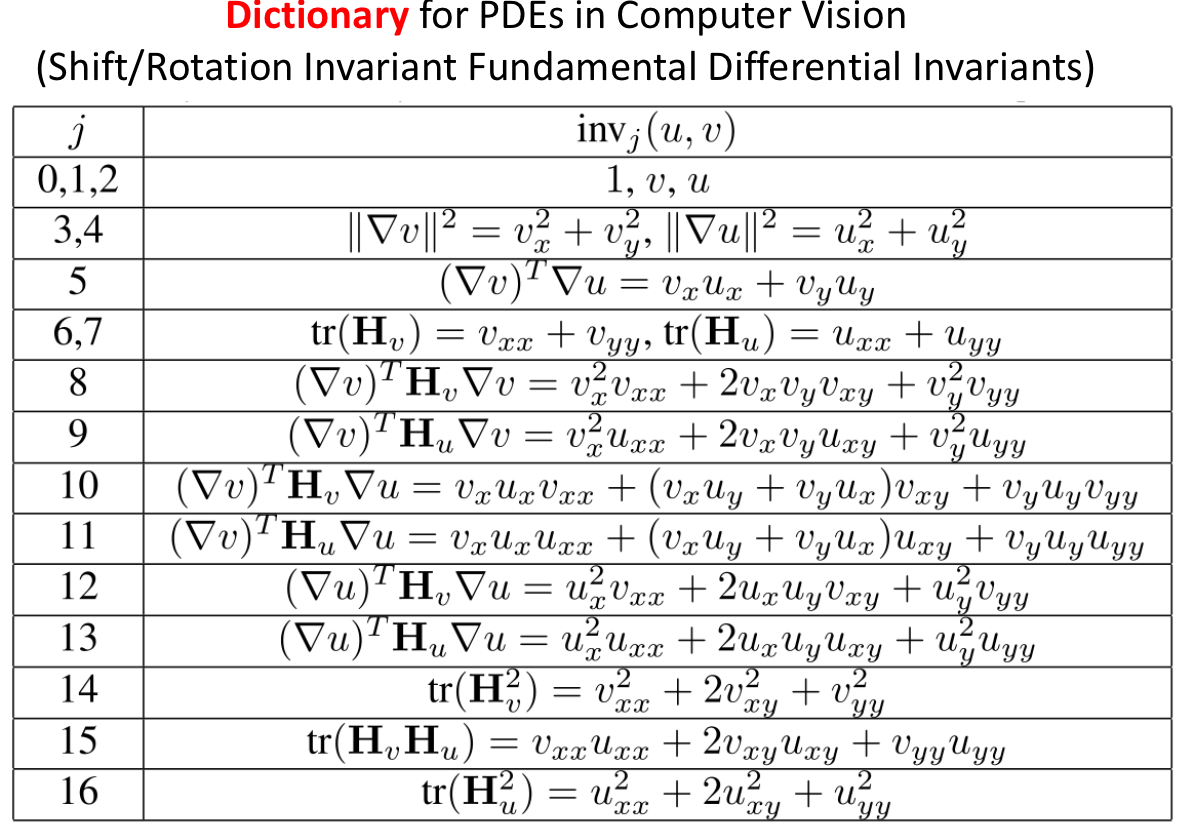
\includegraphics[width=10cm]{dict.png}
\end{figure}

\end{frame}


%
\begin{frame}
\frametitle{几点总结}
关于general PDE system
\begin{itemize}
\item 应用在多方面:图像去噪,边缘检测,模糊与去模糊,图像分割等
\item 高阶PDE,复杂的组合-多层PDE系统
\item 更精确的理论解求解方法
\end{itemize}

\end{frame}

%
\begin{frame}
\frametitle{几点总结}
\begin{itemize}
\item 一般性的PDE或具体的PDE
\item 物理意义,其他
\item 与deep learning的潜在联系
\item $\cdots$
\end{itemize}
\end{frame}




\end{document}
